% ============================================================
% appendix.tex — 附录
% ============================================================

\chapter{补充材料}

% ============================================================
\section{评测协议、环境与复现入口}
\label{sec:app-fp16-protocol}
\label{sec:app-ppl-baseline-matrix}
% ============================================================

本节汇总三类复现审计材料：PPL 评测协议与 FP16 基线、
软硬件环境，以及主线实验的复现入口与覆盖范围。
这些信息用于解释正文表格的协议边界与复现条件，
不承担新的实验结论。

\paragraph{PPL 协议与基线。}
本文 PPL 评测在不同章节使用了三种略有差异的协议，
表~\ref{tab:app-ppl-baseline-matrix} 统一列出各模型 FP16 PPL 基线与对应协议，
供读者在交叉比较时参照。
同一模型同一精度在不同协议下可能出现 $\sim$0.1--0.5 PPL 差异，
各表的\emph{绝对}数字不可直接跨表比较；
各退化率（相对同表内 FP16 基线）方可在表内对比。

\begin{table}[!htbp]
  \centering
  \caption{FP16 PPL 基线 $\times$ 评测协议汇总。}
  \label{tab:app-ppl-baseline-matrix}
  \small
  \begin{threeparttable}
  \begin{tabular}{llccl}
    \toprule
    模型 & 协议 & \code{max\_length} / stride & \code{chunk\_size} & FP16 PPL \\
    \midrule
    Qwen2.5-1.5B & 32K 上下文短窗   & 1024 / 512 & 128 & 8.93 \\
    Qwen2.5-1.5B & 完整 test split  & 32K / 32K  & 128 & 9.31 \\
    Qwen2.5-7B   & 32K 上下文短窗   & 1024 / 512 & 128 & 6.71 \\
    Qwen2.5-7B   & 完整 test split  & 32K / 32K  & 128 & 7.14 \\
    Qwen2.5-7B   & KL/MSE 配对诊断子集 & 32K / 32K & 128 & 6.7097\tnote{$\dagger$} \\
    LLaMA-3.1-8B & 32K 上下文短窗   & 1024 / 512 & 128 & 6.92 \\
    LLaMA-3.1-8B & 完整 test split  & 32K / 32K  & 128 & 6.73 \\
    Qwen2.5-14B  & 32K prefix       & 32K / ---  & 128 & 4.685\tnote{$\star$} \\
    \bottomrule
  \end{tabular}
  \begin{tablenotes}
  \footnotesize
  \item[$\dagger$] 附录表~\ref{tab:app-7b-kl-mse} 的 7B FP16 基线 PPL 精确到四位小数为 $6.7097$，
    来自 KL/MSE 校准目标对比使用的配对诊断子集；本表第四行的 $7.14$ 对应完整 test split 汇总口径。
    两者采用相同的 PPL 定义、窗口长度与 \code{chunk\_size}，但样本覆盖与聚合人口不同，因此只允许在各自协议内部进行配对比较，不作为跨表绝对值比较对象。该表对比 INT4 KL/MSE 校准在 7B 上产生的\emph{逐位一致} PPL（$7.1121$，属 INT4 侧观察，非 FP16 基线）。
  \item[$\star$] 14B 因 H20 显存限制仅在 test split 前 32767 tokens 上评测，
    与其他模型的完整 $\sim$302K test split 不可直接比较。
  \end{tablenotes}
  \end{threeparttable}
\end{table}

\noindent
注：表~\ref{tab:t3-cross-model-main} 与附录第~\ref{sec:app-kv-ablation-full}~节使用 32K 上下文短窗协议；
表~\ref{tab:t2-int4-kivi} 使用完整 test split。

\phantomsection
\paragraph{实验环境。}
\label{sec:app-env}

表~\ref{tab:app-env} 列出了本文所有实验所使用的软硬件环境配置。

\begin{table}[!htbp]
  \centering
  \caption{实验软硬件环境}
  \label{tab:app-env}
  \begin{tabular}{ll}
    \toprule
    \textbf{项目} & \textbf{配置} \\
    \midrule
    GPU             & NVIDIA H20, 98\,GB HBM \\
    CPU             & Intel Xeon \\
    操作系统        & Ubuntu 22.04 LTS \\
    Python          & 3.12 \\
    PyTorch         & 2.8.0 (CUDA 12.8) \\
    Transformers    & 4.48+ \\
    Triton          & 3.2+ \\
    NumPy           & 2.x \\
    pandas          & 2.x \\
    Matplotlib      & 3.x \\
    \bottomrule
  \end{tabular}
\end{table}

生成式质量评测采用固定随机种子（主实验 1234--1238）与贪心解码策略（\code{temperature=0.0}, \code{top\_p=1.0}, \code{top\_k=0}），吞吐实验采用固定随机种子 1234--1241，以确保结果的可复现性。
PPL 采用固定输入序列上的 likelihood 累计，seed 仅用于实现路径一致性核验，不作为统计重复，也不绑定上述生成式解码设置。

\phantomsection
\paragraph{复现入口与覆盖范围。}
\label{sec:app-reproduce}

本文主线实验保留了一套公开复现配置与 artifact 清单。
对应条目覆盖第四章的基准路径验证、低比特恢复、
跨模型预算分配与第~\ref{sec:exp-deployment}~节的部署效率评估，
并补充附录 \ref{subsec:app-7b-kl-mse} 的 7B KL/MSE 趋同溯源。
BitDecoding 案例与官方 LongBench v2 数据作为补充参考材料保留，
但不在主线复现保证范围内。

关于校准样本数量：表~\ref{tab:app-search-space} 中的 $N=128$
表示正文口径下的标准规模，复现配置实际使用
$N\in\{16, 32\}$ 来复现同一已选参数配置。
校准样本数量敏感性检查（覆盖 $s\in\{16, 64, 256\}$）
确认 PPL/Needle/RULER/LongBench 四类指标均已进入平坦收敛域。

% ============================================================
\section{量化路径与复现配置类别}
\label{sec:app-kv-modes}
% ============================================================

本节只承担复现审计的论文侧说明。
表~\ref{tab:ch3-kv-modes} 给出正文量化路径名称与复现配置类别之间的对应关系；
具体配置键值保留在公开 artifact manifest 中，正文论证只使用左列名称。

\begin{table}[!htbp]
  \centering
  \caption{正文量化路径与复现配置类别的对应关系}
  \label{tab:ch3-kv-modes}
  \scriptsize
  \begin{threeparttable}
  \setlength{\tabcolsep}{3pt}
  \renewcommand{\arraystretch}{1.08}
  \begin{tabularx}{\linewidth}{p{2.45cm}p{2.75cm}cp{2.05cm}X}
    \toprule
    \textbf{正文名称} & \textbf{复现配置类别} & \textbf{K/V 位宽} & \textbf{默认执行路径} & \textbf{说明} \\
    \midrule
    FP16 & full-precision reference & 16/16 & FP16 & 全精度基线 \\
    INT8 baseline & percentile symmetric baseline & 8/8 & \makecell[l]{参考实现 /\\Triton} & percentile 对称基线 \\
    INT8-Canonical & behavior-guided symmetric INT8 & 8/8 & Triton & KL-guided 对称基准路径 \\
    INT4 percentile baseline & percentile symmetric INT4 & 4/4 & 参考实现 & percentile 对称低比特基线 \\
    \makecell[l]{对称 INT4\\(behavior-guided)} & behavior-guided symmetric INT4 & 4/4 & 参考实现 & KL-guided 对称 INT4 \\
    \makecell[l]{融合 INT4\\诊断变体} & symmetric INT4 fused-kernel diagnostic & 4/4 & Triton & 同校准参数的融合路径诊断，非 Ch4 主表项 \\
    INT4-RoleAlign & role-aware asymmetric INT4 & 4/4 & 参考实现\tnote{$\star$} & per-channel K + per-token V \\
    KIVI-style & runtime-statistic asymmetric INT4 & 4/4 & 参考实现 & 同格式 runtime 统计基线 \\
    MixedKV & mixed-precision diagnostic & 8/4 & 参考实现 & K8V4 诊断路径 \\
    \bottomrule
  \end{tabularx}
  \begin{tablenotes}
    \small
    \item 注：第四章主表使用左列正文名称；中列仅说明公开复现材料中的配置类别，不作为正文方法命名。
    INT4-RoleAlign 与 KIVI-style 共享 per-channel K + per-token V 缓存格式，
    二者差异限定在离线行为校准与运行时统计更新的参数来源上。
    \item[$\star$] INT4-RoleAlign 的非对称 Triton 变体只作为实现可行性验证；
    正文质量评测默认使用参考解码实现，系统讨论见第~\ref{sec:exp-deployment}~节。
  \end{tablenotes}
  \end{threeparttable}
\end{table}

% ============================================================
\section{校准产物与搜索空间审计}
\label{sec:app-calib-schema}
% ============================================================

离线校准阶段产出一份小型结构化校准记录（$<$10~KB），
其中包含路径特定的逐层 Key/Value scale、zero point、
分位数参数、分组元数据，以及模型标识、校准样本数、seed、目标函数与量化格式等审计字段。
对称路径主要消费静态 scale 与分组参数；
INT4-RoleAlign 额外记录 per-channel Key 与 per-token Value 的角色感知分位数参数。
逐头温度校正字段若出现在早期诊断记录中，仅用于附录第~\ref{sec:app-invtau-diagnostic}~节的诊断复现；
第三章与第四章主线配置不使用该组件。
推理时一次性加载相应产物到 GPU 显存，不引入运行时校准开销。

\phantomsection
\paragraph{校准超参数搜索空间。}
\label{sec:app-calib-search-space}

表~\ref{tab:app-search-space} 汇总主线校准搜索空间；对称量化数据结构只保留复现所需常量。

\begin{table}[!htbp]
  \centering
  \caption{校准超参数搜索空间}
  \label{tab:app-search-space}
  \small
  \begin{tabular}{lll}
    \toprule
    超参数 & 符号 & 候选值集合 / 默认配置 \\
    \midrule
    \multicolumn{3}{l}{\textit{对称格式常量}} \\
    位宽 / 范围 & $n, q_{\max}$ & INT8: 8 / 127；INT4: 4 / 7 \\
    Scale / 量化轴 & --- & float32 scale，对称 per-group（沿 $d_k$ 分组） \\
    \midrule
    \multicolumn{3}{l}{\textit{INT8 对称量化路径（主线校准搜索）}} \\
    Clip percentile & $\mathcal{P}_c$ & $\{99.0,\; 99.5,\; 99.9,\; 100.0\}$（默认 99.5） \\
    Group size & $\mathcal{G}$ & $\{16,\; 32,\; 64,\; 128\}$（默认 16） \\
    Outlier rescue ratio & --- & $\{0,\; 0.0025,\; 0.005,\; 0.01\}$ \\
    \midrule
    \multicolumn{3}{l}{\textit{补充诊断分支}} \\
    温度因子 & $\mathcal{T}$ & $\{0.5,\; 0.7,\; 0.85,\; 1.0,\; 1.2,\; 1.5,\; 2.0\}$（不计入主线搜索规模） \\
    \midrule
    \multicolumn{3}{l}{\textit{INT4-RoleAlign 非对称量化路径}} \\
    K percentile & $\mathcal{P}_K$ & $\{95.0,\; 97.0,\; 99.0,\; 99.5,\; 99.9,\; 100.0\}$ \\
    V percentile & $\mathcal{P}_V$ & $\{95.0,\; 97.0,\; 99.0,\; 99.5,\; 99.9,\; 100.0\}$ \\
    \midrule
    共用参数 & $N$, len, data & 128（标准规模）；512 tokens；WikiText-2 (test split) \\
    \bottomrule
  \end{tabular}
\end{table}

其中 $N=128$ 表示正文口径下的标准校准规模；复现配置使用
$N\in\{16,32\}$ 复现同一已选参数配置，见附录第~\ref{sec:app-reproduce}~节说明。
INT8 基准路径主线搜索为 $|\mathcal{P}_c| \times |\mathcal{G}| = 16$ 组；温度因子只属补充诊断，不计入搜索规模，也不改变主线默认配置。
INT4-RoleAlign 可枚举 $|\mathcal{P}_K| \times |\mathcal{P}_V| = 36$ 组用于审计，但 K-path 与 V-path 的代理需分别解释。

% ============================================================
\section{LongBench、统计检验与质量趋势补充材料}
\label{sec:app-longbench-full}
% ============================================================

本节合并三类质量补充材料：LongBench-style 合成评测的完整审计表、
官方 LongBench 小范围协议一致性检查、以及统计检验与上下文长度趋势图。
这些材料共同服务于第四章的可信性边界，而不替代正文主表或扩大主结论适用范围。

\paragraph{LongBench-style 补充聚合表。}
表~\ref{tab:app-longbench-full} 列出了三种模型在 32K 上下文长度下、七种实验路径的
LongBench-style 聚合结果，包含 F1 宏平均、包含匹配宏平均以及综合评分。
数值后的``$\pm$''表示 Bootstrap 95\% 置信区间半宽。
本表只作为正文基准保真与低比特恢复证据的补充审计材料；
其中 8B 的 INT4 读数不应被反向概括为低比特路径普遍安全。

\begin{table}[!htbp]
  \centering
  \begin{threeparttable}
  \caption{LongBench-style 补充聚合结果（32K 上下文，三模型 $\times$ 七实验路径）}
  \label{tab:app-longbench-full}
  \zihao{5}
  \begin{tabular}{lp{3.4cm}rrr}
    \toprule
    \textbf{模型} & \textbf{实验路径} & \textbf{F1 宏平均} & \textbf{包含匹配率(\%)} & \textbf{综合评分} \\
    \midrule
    \multirow{7}{*}{1.5B}
      & FP16                         & $5.53 \pm 0.05$ & $99.9 \pm 0.2$ & $0.0482 \pm 0.0004$ \\
      & INT8-Baseline                & $5.50 \pm 0.02$ & $99.9 \pm 0.2$ & $0.0478 \pm 0.0002$ \\
      & INT8-Canonical               & $5.54 \pm 0.04$ & $99.9 \pm 0.1$ & $0.0482 \pm 0.0004$ \\
      & INT4 percentile              & $2.91 \pm 0.26$ & $45.9 \pm 2.0$ & $0.0298 \pm 0.0024$ \\
      & Fused INT4                   & $0.00 \pm 0.00$ & $0.0 \pm 0.0$  & $0.0515 \pm 0.0068$ \\
      & Behavior-guided INT4         & $0.00 \pm 0.00$ & $0.0 \pm 0.0$  & $0.0241 \pm 0.0025$ \\
      & KIVI-style                   & $5.58 \pm 0.07$ & $99.9 \pm 0.1$ & $0.0481 \pm 0.0005$ \\
    \midrule
    \multirow{7}{*}{7B}
      & FP16                         & $4.29 \pm 0.15$ & $100.0 \pm 0.0$ & $0.0378 \pm 0.0008$ \\
      & INT8-Baseline                & $4.38 \pm 0.14$ & $100.0 \pm 0.0$ & $0.0383 \pm 0.0007$ \\
      & INT8-Canonical               & $4.44 \pm 0.14$ & $100.0 \pm 0.0$ & $0.0383 \pm 0.0009$ \\
      & INT4 percentile              & $0.00 \pm 0.00$ & $0.0 \pm 0.0$   & $0.0172 \pm 0.0024$ \\
      & Fused INT4                   & $0.45 \pm 0.13$ & $4.2 \pm 0.9$   & $0.0183 \pm 0.0020$ \\
      & Behavior-guided INT4         & $0.00 \pm 0.01$ & $0.4 \pm 0.5$   & $0.0027 \pm 0.0011$ \\
      & KIVI-style                   & $4.28 \pm 0.14$ & $99.9 \pm 0.1$  & $0.0378 \pm 0.0011$ \\
    \midrule
    \multirow{7}{*}{8B}
      & FP16                         & $10.29 \pm 0.76$ & $99.7 \pm 0.5$ & $0.0792 \pm 0.0066$ \\
      & INT8-Baseline                & $10.71 \pm 0.85$ & $99.7 \pm 0.5$ & $0.0817 \pm 0.0092$ \\
      & INT8-Canonical               & $10.72 \pm 0.85$ & $99.6 \pm 0.7$ & $0.0817 \pm 0.0092$ \\
      & INT4 percentile              & $12.95 \pm 1.02$ & $99.7 \pm 0.5$ & $0.1037 \pm 0.0087$ \\
      & Fused INT4                   & $15.89 \pm 1.37$ & $99.8 \pm 0.3$ & $0.1505 \pm 0.0138$ \\
      & Behavior-guided INT4         & $19.88 \pm 1.34$ & $99.4 \pm 0.5$ & $0.1908 \pm 0.0111$ \\
      & KIVI-style                   & $8.72 \pm 0.98$  & $99.6 \pm 0.3$ & $0.0682 \pm 0.0069$ \\
    \bottomrule
  \end{tabular}
  \begin{tablenotes}
    \footnotesize
    \item 注：1.5B = Qwen2.5-1.5B-Instruct，
    7B = Qwen2.5-7B-Instruct，
    8B = LLaMA-3.1-8B-Instruct。
    合成 LongBench（7 类子任务），5 seeds 均值。
    8B INT4 的较高 F1 可能反映合成任务、评分器或该模型/路径组合下的协议特异性，
    不作为 INT4 优于 FP16 或 KIVI-style 的主证据。
  \end{tablenotes}
  \end{threeparttable}
\end{table}

% Compatibility anchors retained after merging former A.7--A.9 sections.
\phantomsection
\paragraph{官方数据一致性检查。}
\label{sec:app-longbench-official}
前述 LongBench-style 评测使用确定性合成数据源，
绝对值不可与社区官方榜单直接对齐。
为检查主评测协议是否存在方向性误判，
本文在 LongBench~\cite{bai2024longbench} 官方数据集上使用 Qwen2.5-1.5B-Instruct、
32K 截断、seed=1234 和每任务最多 50 个样本，
选取 NarrativeQA、HotpotQA 与 GovReport 三个任务做小范围对照。
在 INT8-Canonical 相对 FP16 的比较中，
三项差异分别为 $-0.43$、$+0.31$、$+0.08$ pp，
宏平均为 FP16=$7.06$、INT8-Canonical=$7.05$。
这一小范围官方对照与合成协议对 INT8 基准路径保真方向的判断保持一致，
其作用限定在协议一致性检查层面。

\phantomsection
\paragraph{统计检验设置与结果。}
\label{sec:app-seed-detail}

表~\ref{tab:app-sig-quality} 合并列出了 INT8 路径在固定序列 PPL、生成式质量指标
（Needle/LongBench/RULER，$n=5$ 种子）与推理延迟
（TPOT，$n=8$ 种子）上的审计结果。
PPL 行对应固定输入序列上的 likelihood 累计，只报告效应量，不进入显著性检验；
Needle 行对应主配置，LongBench 与 RULER 行使用主配置及补充配置的合并读数，
因此只用于稳定性审计，不作为正文主路径 claim。
生成式质量指标与延迟指标的检验均基于配对种子的 sign-flip 置换检验，
多重比较校正采用 Benjamini-Hochberg FDR 控制（$\alpha=0.05$）。

\begin{table}[!htbp]
  \centering
  \caption{INT8 固定序列 PPL、质量与延迟审计统计（32K 上下文）}
  \label{tab:app-sig-quality}
  \zihao{5}
  \begin{tabular}{llrrrrrr}
    \toprule
    \textbf{模型} & \textbf{指标} & \textbf{INT8-Baseline} & \textbf{审计对象} & \textbf{变化(\%)} & \textbf{$p$值} & \textbf{$q$值} & \textbf{显著} \\
    \midrule
    \multicolumn{8}{l}{\textit{固定序列 PPL（不做显著性检验）}} \\
    \midrule
    1.5B & PPL$\downarrow$             & 8.9316 & 8.9497 & $-0.20$ & N/A & N/A & N/A \\
    7B   & PPL$\downarrow$             & 6.7145 & 6.7322 & $-0.26$ & N/A & N/A & N/A \\
    8B   & PPL$\downarrow$             & 6.9193 & 6.9252 & $-0.09$ & N/A & N/A & N/A \\
    \midrule
    \multicolumn{8}{l}{\textit{生成式质量指标（$n=5$ 种子 1234--1238）}} \\
    \midrule
    \multirow{3}{*}{1.5B}
      & Needle pass rate$\uparrow$   & 100.00 & 100.00 & $+0.00$ & 1.0000 & 1.0000 & 否 \\
      & LongBench score$\uparrow$    & 0.0478 & 0.0486 & $+1.77$ & 0.0909 & 0.1435 & 否 \\
      & RULER pass rate$\uparrow$    & 24.45  & 23.81  & $-2.64$ & 0.0909 & 0.7273 & 否 \\
    \midrule
    \multirow{3}{*}{7B}
      & Needle pass rate$\uparrow$   & 100.00 & 100.00 & $+0.00$ & 1.0000 & 1.0000 & 否 \\
      & LongBench score$\uparrow$    & 0.0383 & 0.0383 & $+0.17$ & 0.9394 & 0.9553 & 否 \\
      & RULER pass rate$\uparrow$    & 24.92  & 24.84  & $-0.31$ & 1.0000 & 1.0000 & 否 \\
    \midrule
    \multirow{3}{*}{8B}
      & Needle pass rate$\uparrow$   & 100.00 & 100.00 & $+0.00$ & 1.0000 & 1.0000 & 否 \\
      & LongBench score$\uparrow$    & 0.0817 & 0.0817 & $+0.09$ & 0.8788 & 0.9416 & 否 \\
      & RULER pass rate$\uparrow$    & 32.58  & 31.25  & $-4.05$ & 0.0909 & 0.7273 & 否 \\
    \midrule
    \multicolumn{8}{l}{\textit{解码延迟 TPOT（$n=8$ 种子 1234--1241，batch size 为 1，生成长度为 64 tokens）}} \\
    \midrule
    1.5B & TPOT (ms)$\downarrow$ & 51.42 & 47.14 & $+8.32$  & 0.0117 & 0.0159 & \textbf{是} \\
    7B   & TPOT (ms)$\downarrow$ & 60.52 & 50.07 & $+17.26$ & 0.0117 & 0.0159 & \textbf{是} \\
    8B   & TPOT (ms)$\downarrow$ & 91.77 & 57.23 & $+37.64$ & 0.0117 & 0.0159 & \textbf{是} \\
    \bottomrule
  \end{tabular}

  \vspace{2pt}
  {\footnotesize 注：PPL 为固定输入序列上的确定性 likelihood 指标，seed 只用于实现路径一致性核验，因此不进入生成式指标的显著性检验流程。
  生成式质量指标差异均未达到 BH-FDR 校正后的统计显著性；三种模型上的 TPOT 降低均达到显著性（$q < 0.05$）。1.5B Needle 行报告主配置（5 种子均 100\%）；LongBench/RULER 行为主配置与补充配置的合并审计读数，其中 RULER 退化主要受补充配置影响。}
\end{table}

\phantomsection
\paragraph{上下文长度质量趋势表。}
\label{sec:app-quality-plots}

表~\ref{tab:app-quality-context-summary} 汇总了 Qwen2.5-1.5B-Instruct 上 RULER 与
LongBench-style 综合评分在不同上下文长度下的关键读数。
该表只保留 FP16 与 INT8-Canonical 两条主线参照，用于确认补充质量指标没有改变正文主结论；
低比特长上下文边界则由图~\ref{fig:app-needle-depth-grid}
和附录第~\ref{sec:app-int4-mechanism-boundary}~节补充。

\begin{table}[!htbp]
  \centering
  \caption{补充质量指标随上下文长度的关键读数（Qwen2.5-1.5B-Instruct）。}
  \label{tab:app-quality-context-summary}
  \scriptsize
  \setlength{\tabcolsep}{4pt}
  \begin{tabular}{@{}lcccc@{}}
    \toprule
    \textbf{上下文长度} & \makecell{\textbf{RULER}\\\textbf{FP16}}
      & \makecell{\textbf{RULER}\\\textbf{INT8-Canonical}}
      & \makecell{\textbf{LongBench}\\\textbf{FP16}}
      & \makecell{\textbf{LongBench}\\\textbf{INT8-Canonical}} \\
    \midrule
    4K  & 24.84 & 24.87 & 4.37 & 4.51 \\
    8K  & 24.92 & 24.92 & 4.82 & 5.00 \\
    16K & 24.77 & 24.84 & 4.82 & 5.00 \\
    32K & 24.38 & 23.88 & 4.82 & 4.92 \\
    \bottomrule
  \end{tabular}

  \vspace{2pt}
  {\footnotesize 注：RULER 为通过率（\%）；LongBench-style 综合评分按 $\times 100$ 报告。}
\end{table}

% ============================================================
\section{部署效率与批处理扩展补充}
\label{sec:app-efficiency-plots}
% ============================================================

本节汇总 Qwen2.5-1.5B-Instruct 上的系统补充读数，
包括单序列 TPOT 边界说明、吞吐/显存扩展图，以及 batch 维度的容量边界。
这些材料只服务于第~\ref{sec:exp-deployment}~节的部署边界审计；
硬件、后端路径、batch size 与序列长度条件均不应外推为通用速度结论。

\paragraph{单序列 TPOT 边界与资源扩展图。}
单序列 TPOT 读数在下文以文字说明；
图~\ref{fig:app-throughput-dashboard} 和图~\ref{fig:app-memory-dashboard}
分别补充展示吞吐与显存扩展读数。

单序列 TPOT 的补充读数显示，在 Qwen2.5-1.5B-Instruct、NVIDIA H20、batch=1 的设置下，
量化路径仍受到固定开销约束，适合作为部署边界条件的说明。
第~\ref{sec:exp-deployment}~节的部署结论仍以正文表~\ref{tab:ch4-tpot-4k}
--\ref{tab:ch4-kvcache-memory} 以及本节的吞吐、显存补充读数为准。

\begin{figure}[!htbp]
  \centering
  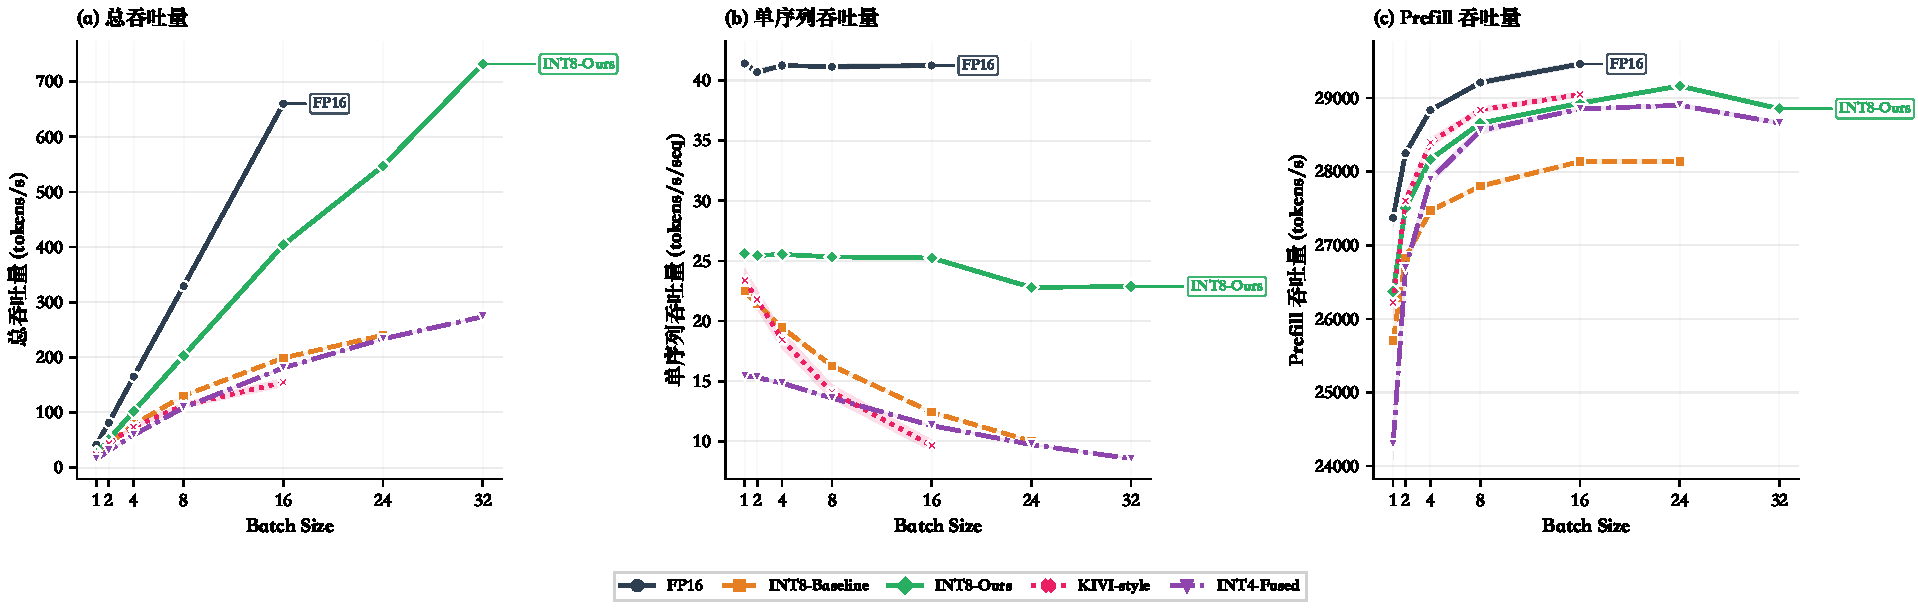
\includegraphics[width=0.9\textwidth]{figures/appendix_throughput_dashboard.pdf}
  \caption{吞吐扩展性三联图（Qwen2.5-1.5B-Instruct，NVIDIA H20，序列长度 8192，生成长度 128）。
  面板（a）展示总吞吐量，面板（b）展示单序列吞吐量，
  面板（c）展示 prefill 吞吐量。统一图例和坐标轴用于观察当前后端组合下 batch 扩展中的并发收益与单序列代价。}
  \label{fig:app-throughput-dashboard}
\end{figure}

\begin{figure}[!htbp]
  \centering
  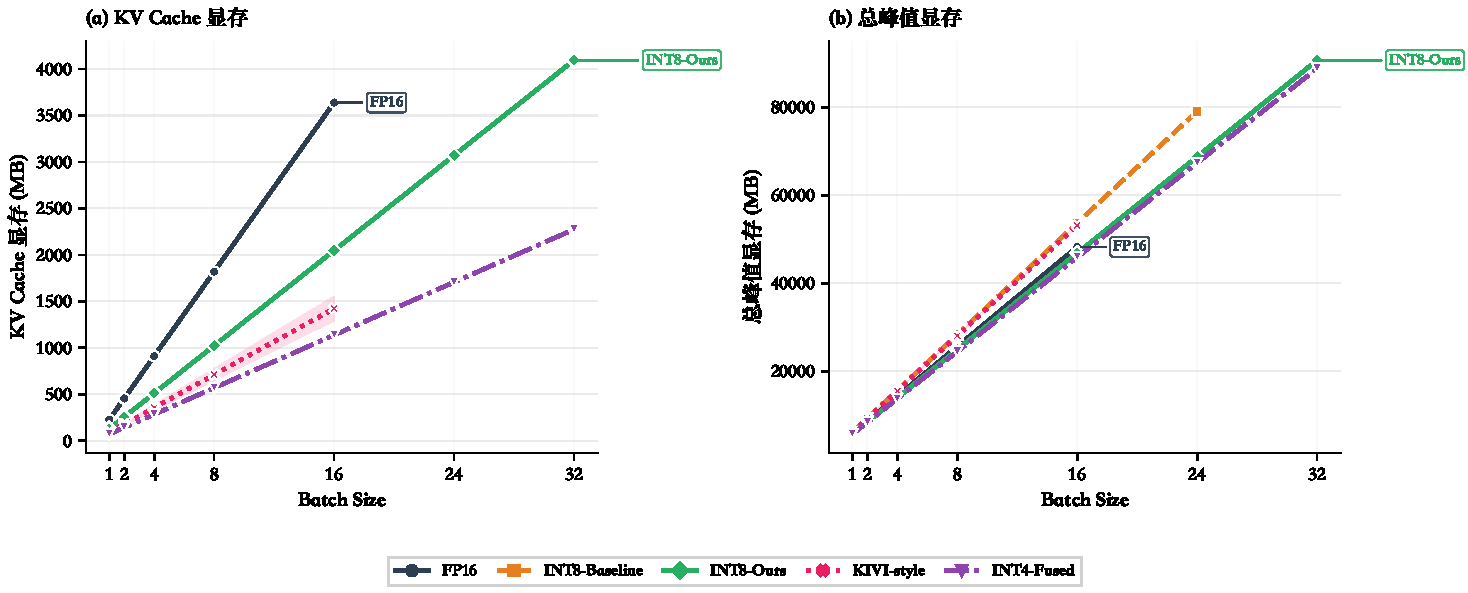
\includegraphics[width=0.9\textwidth]{figures/appendix_memory_dashboard.pdf}
  \caption{显存扩展性双联图（Qwen2.5-1.5B-Instruct，NVIDIA H20，序列长度 8192）。
  面板（a）展示 KV Cache 显存随 batch size 的线性增长，
  面板（b）展示总峰值显存；两者共同说明量化节省如何改变当前扫描范围内的可容纳 batch。}
  \label{fig:app-memory-dashboard}
\end{figure}

\phantomsection
\paragraph{批处理容量与 INT4-RoleAlign 扩展轨迹。}
\label{sec:app-batch-capacity}

表~\ref{tab:app-batch} 合并呈现 batch 维度的容量边界与扩展轨迹：
（a）各模式在序列长度 8192 条件下的已测最大可行 batch；
（b）INT4-RoleAlign 在不同 batch 下的 TPOT 与 KV Cache 显存。

\begin{table}[!htbp]
  \centering
  \caption{批处理扩展综合数据（Qwen2.5-1.5B-Instruct，NVIDIA H20，序列长度 8192，独占 GPU）}
  \label{tab:app-batch}
  \small
  \resizebox{\textwidth}{!}{%
  \begin{tabular}{lccc}
    \toprule
    \multicolumn{4}{l}{\textit{（a）各量化模式已测最大可行 batch（1--32 扫描）}} \\
    \midrule
    \textbf{量化模式} & \textbf{已测最大可行 batch} & \textbf{扫描范围} & \textbf{容量结论} \\
    \midrule
    FP16            & 16 & 1--16 & 范围内可行；未扩展至 32 \\
    INT8-Baseline   & 24 & 1--32 & batch=32 显存不足 \\
    INT8-Canonical  & 32 & 1--32 & 范围内可行 \\
    INT4-Baseline   & 16 & 1--16 & 范围内可行；未扩展至 32 \\
    INT4-Fused      & 32 & 1--32 & 范围内可行 \\
    INT4-RoleAlign  & 32 & 1--32 & 范围内可行 \\
    \midrule
    \multicolumn{4}{l}{\textit{（b）INT4-RoleAlign 批处理扩展轨迹（FP16 vs INT4-RA 对照）}} \\
    \midrule
    \textbf{Batch} & \textbf{TPOT FP16 / INT4-RA (ms)} & \textbf{KV FP16 / INT4-RA (MB)} & \textbf{KV 压缩比} \\
    \midrule
    1  & 24.78 / 60.18  & 227  / 60  & 3.78$\times$ \\
    4  & 24.65 / 73.17  & 910  / 242 & 3.76$\times$ \\
    8  & 24.21 / 93.07  & 1820 / 484 & 3.76$\times$ \\
    16 & 24.23 / 134.46 & 3640 / 968 & 3.76$\times$ \\
    \bottomrule
  \end{tabular}
  }

  \vspace{2pt}
  {\footnotesize 注：（a）在序列长度 8192、NVIDIA H20 与当前后端组合下，INT8-Canonical 与 INT4 融合模式均可支持已测 batch=32；INT8-Baseline 在 batch=32 时出现中间张量显存不足，因此容量边界从 24 移至 32 只相对于该 baseline 解释。（b）KV 压缩比约 3.76$\times$ 恒定；INT4-RoleAlign 的 TPOT 随 batch 增长，说明该实现仍有并发反量化摊销开销。batch=16 时其 KV Cache 为 968~MB（FP16 为 3640~MB），主要收益体现在容量边界而非速度主结论。}
\end{table}

% Supplementary deployment diagnostics.

% ============================================================
\section{INT4 失稳机制与评估粒度边界补充}
\label{sec:app-int4-mechanism-boundary}
% ============================================================

本节按四层组织 INT4 相关补充材料：首先用 Needle 深度--位置热力图给出
long-context cliff 的可视化背景；随后用 scale 精度敏感性读数排除
“scale dtype 单点失误”解释；第三部分保留噪声--长度交互的近似推导，给出
32K 场景下 INT4 阶跃退化的机制直觉；最后用 chunk size 消融界定评估粒度和
流式近似协议边界。最后一部分只限定协议适用范围，不引入新的主机制结论。

\phantomsection
\paragraph{Needle 深度--位置热力图补充。}
\label{sec:app-needle-heatmaps}
图~\ref{fig:app-needle-depth-grid} 补充展示 Needle 任务的深度位置热力图。
该图服务于正文第~\ref{subsec:ch4-int4-cliff}~节的阶跃崩塌模式：
它说明在当前热力图覆盖设置下，对称 INT4 的退化主要在长上下文与深层 needle 位置上被放大，
并为下文噪声--长度推导提供可视化背景。

\begin{figure}[!htbp]
  \centering
  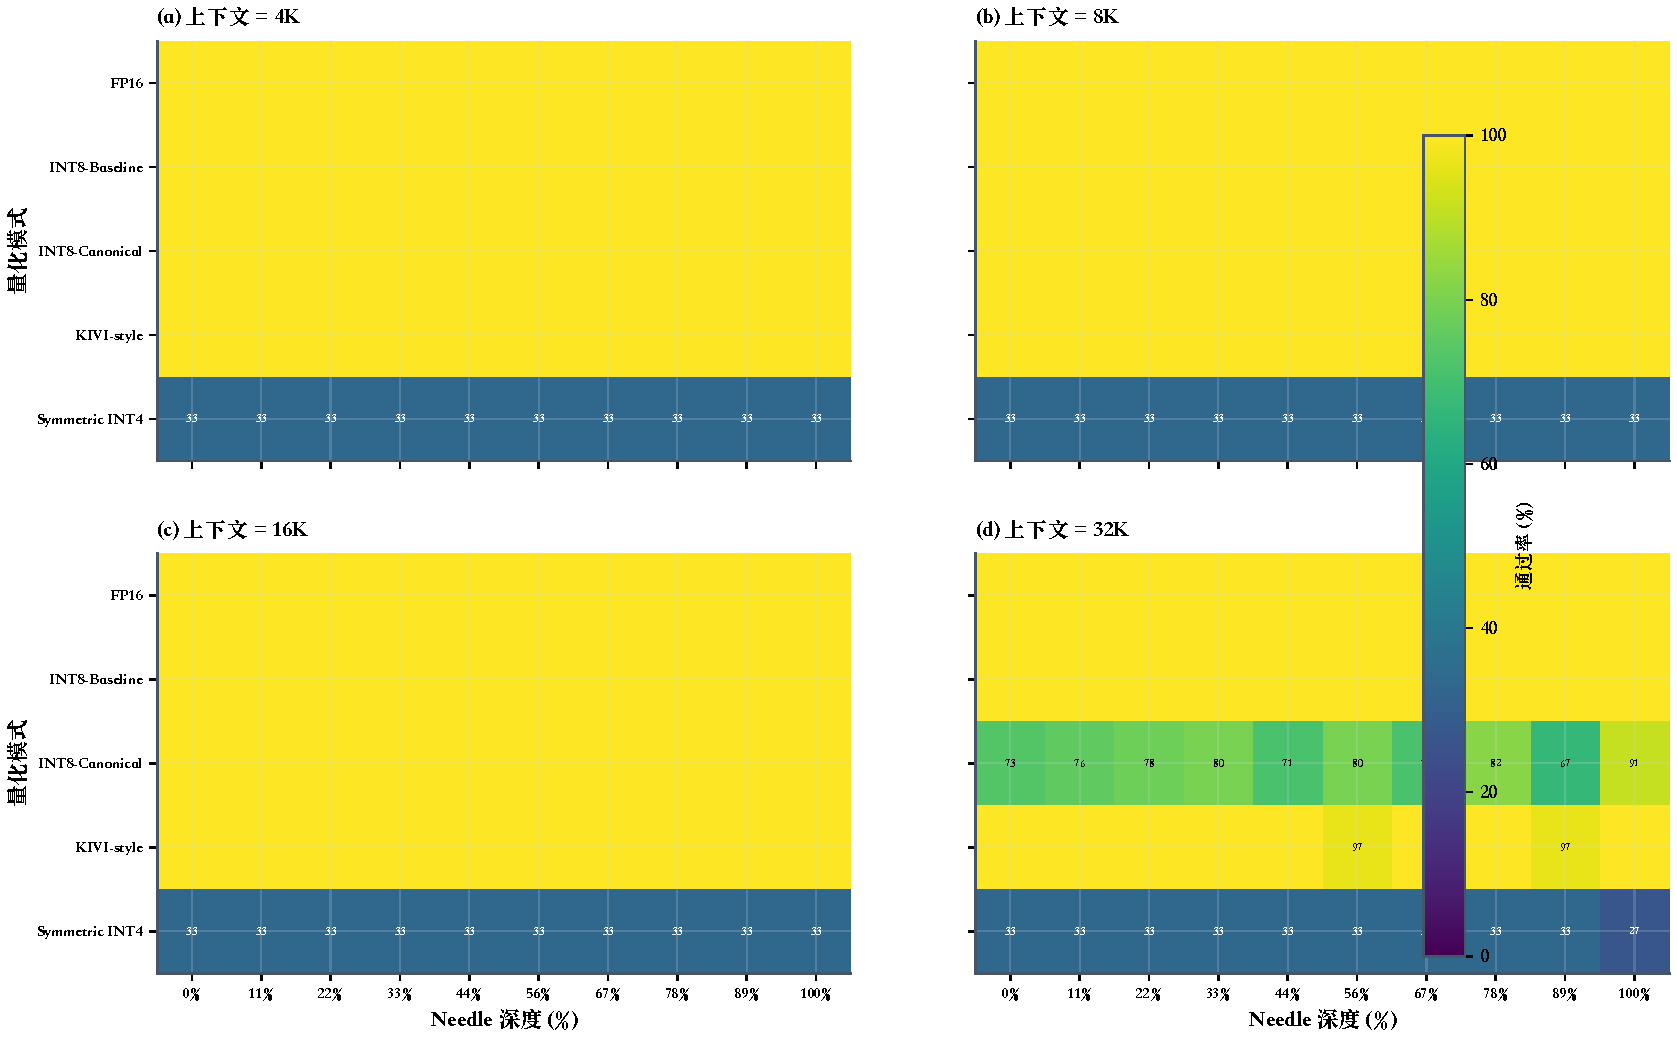
\includegraphics[width=\textwidth]{figures/needle_depth_grid.pdf}
  \caption{Needle-in-a-Haystack 深度-位置热力图总览。
  四个面板分别对应 4K、8K、16K 和 32K，并共享同一色标。
  该图用于定位 INT4 退化在上下文长度和 needle 深度上的放大位置，
  不替代正文的主表结论。}
  \label{fig:app-needle-depth-grid}
\end{figure}

精确匹配率（exact match）采用比通过率更严格的 Needle 判据，
其趋势与图~\ref{fig:app-needle-depth-grid} 一致：
FP16 在 4K--32K 均保持 100\%，INT8-Canonical 在 4K--16K 保持 100\%，
并在 32K 端点给出约 70.3\% 的长上下文边界读数；
对称 INT4 则在 4K 已显露边界，并在 8K 及以上区间构成长上下文边界对照。
这些 exact-match 读数作为严格判据补充图~\ref{fig:app-needle-depth-grid}，
不再作为独立视觉证据展开。

\paragraph{Scale 精度敏感性诊断。}
\label{sec:app-scale-precision}
表~\ref{tab:app-scale-precision} 是一组补充诊断读数，用于确认对称 INT4 失稳并非仅由
scale 存储精度不足造成。所有 scale 参数均以 float32 精度维护。
本节中的 behavior-guided 对称 INT4 不等同于正文主线的 INT4-RoleAlign 非对称路径。

\begin{table}[!htbp]
  \centering
  \caption{INT4 量化 scale 精度敏感性实验
    （32K 序列；PPL 为固定序列 likelihood，Needle 使用三个固定种子的贪婪生成）}
  \label{tab:app-scale-precision}
  \resizebox{\textwidth}{!}{%
  \begin{tabular}{llcccc}
    \toprule
    \textbf{模型} & \textbf{模式} & \textbf{PPL} & \textbf{Needle (\%)} & \textbf{校准} & \textbf{Scale dtype} \\
    \midrule
    \multirow{2}{*}{Qwen2.5-1.5B} & Symmetric INT4 baseline & 19.65 & 0 & percentile & float32 \\
                                    & Symmetric INT4 behavior-guided & 22.80 & 0 & KL proxy   & float32 \\
    \midrule
    \multirow{2}{*}{Qwen2.5-7B}   & Symmetric INT4 baseline & 86.56 & --- & percentile & float32 \\
                                    & Symmetric INT4 behavior-guided & 52.19 & --- & KL proxy   & float32 \\
    \midrule
    \multirow{2}{*}{LLaMA-3.1-8B} & Symmetric INT4 baseline & 6.97  & 100 & percentile & float32 \\
                                    & Symmetric INT4 behavior-guided & 7.64  & 100 & KL proxy   & float32 \\
    \bottomrule
  \end{tabular}
  }
  \begin{tablenotes}
    \footnotesize
    \item 注：7B Needle 未包含在该诊断消融中（标记 ---）。
    1.5B Needle 0\% 反映该模型在 32K 对称 INT4 下的边界；
    7B 基线 PPL=86.56 与正文同量级结果一致，说明该敏感性不是 scale dtype 单点造成。
  \end{tablenotes}
\end{table}

\textbf{补充读数。}
在同一 float32 scale 条件下，7B 的 behavior-guided 对称 INT4 PPL 低于 percentile baseline，
但 1.5B 的 Needle 仍为 0\%，LLaMA-3.1-8B 则在两种对称 INT4 配置下保持 100\%。
因此本节只支撑第~\ref{subsec:exp-int4-honest}~节的边界判断：
scale 精度是必要的数值卫生条件，但对称 INT4 cliff 还会受到模型结构与上下文长度调节。

\paragraph{量化噪声与序列长度交互效应。}
\phantomsection
\label{sec:app-sqnr-derivation}
本段提供正文第~\ref{subsec:exp-int4-honest}~节中量化步长与序列长度交互效应的近似分析。

Needle-in-a-Haystack 任务的检索成功条件可形式化为：
目标位置 $t$ 的 attention logit 与最强干扰位置的差值
$\delta = z_t - \max_{i \neq t} z_i$
（其中 $z_i = \bq^\top \bk_i / \sqrt{d_k}$）
需在量化后仍保持正值，使 softmax 将最大概率分配给目标位置。

当 Key 矩阵经 INT4 量化后，每个 logit $z_i$ 受到量化噪声扰动 $\epsilon_i$，
其方差约为：
\begin{equation}
  \text{Var}(\epsilon_i) \approx \|\bq\|^2 \cdot \sigma_{q,4}^2 / d_k
\end{equation}
其中 $\sigma_{q,4}^2 = \Delta_4^2 / 12$ 为 INT4 量化的逐元素噪声方差。

随序列长度 $n$ 增大，$\max_{i \neq t} (z_i + \epsilon_i)$ 的期望值
以 $O(\sqrt{2 \ln n} \cdot \sigma_\epsilon)$ 的速率增长（极值统计理论），
而目标信号 $\delta$ 不随 $n$ 增大。
在这一近似模型下，可以定义一个临界序列长度 $n^*$，满足：
\begin{equation}
  \delta \approx \sqrt{2 \ln n^*} \cdot \sigma_\epsilon
\end{equation}
当 $n > n^*$ 时，量化噪声超过目标 margin 的风险快速上升，检索失败概率随之增大。

在同一对称裁剪范围下，INT8 与 INT4 的 $q_{\max}$ 分别为 127 与 7，
因此 INT4 相对 INT8 的逐元素噪声方差比约为
$\sigma_{q,4}^2 / \sigma_{q,8}^2 = (127/7)^2 \approx 3.29\times 10^2$。
INT4 的 $n^*$ 远小于 INT8。该近似模型为 1.5B 模型上
从短上下文到 32K 的 Needle 通过率下降提供了理论直觉；
实际退化强度仍受模型结构、校准格式和注意力分布共同调节。


\paragraph{评估粒度鲁棒性。}
\phantomsection
\label{sec:app-chunksize}
本段验证量化粒度变化对低比特路径的影响。
前述各节采用 128-token chunk 协议；cs=1 则更接近每步都读写量化历史 KV 的 streaming decode。
表~\ref{tab:app-chunksize} 给出 Qwen2.5-1.5B-Instruct 上
三种粒度下 FP16、\mbox{INT4-RoleAlign} 和 KIVI-style INT4 的 PPL 对比。

\begin{table}[!htbp]
  \centering
  \caption{量化评估粒度敏感性（Qwen2.5-1.5B-Instruct，PPL，seed=1234）}
  \label{tab:app-chunksize}
  \resizebox{\textwidth}{!}{%
  \begin{tabular}{lccc}
    \toprule
    \textbf{配置} & \textbf{cs=128} & \textbf{cs=8} & \textbf{cs=1} \\
    \midrule
    FP16                     & 9.31 & 9.31 & 9.31 \\
    INT8-Canonical           & 8.95 & 9.34 (+0.3\%$^{\dagger}$) & 9.27 (-0.4\%$^{\dagger}$) \\
    \textbf{INT4-RoleAlign}  & \textbf{10.58} (+13.7\%) & \textbf{62.10} (+567\%) & $>$10{,}000$^{\star}$ \\
    KIVI-style INT4          & 10.43 (+12.0\%) & 60.54 (+550\%) & 10{,}332 (+110{,}900\%)$^{\star}$ \\
    \bottomrule
  \end{tabular}%
  }
\end{table}

\noindent\emph{表注与边界。}
括号内为相对 FP16 的 PPL 变化率，cs = chunk\_size。
$^{\dagger}$ INT8-Canonical 的 cs=128 PPL 低于 FP16，主要反映评测切分口径差异；
cs=1 相对 FP16 仍基本持平，说明更高量化级别提供了更大的 range 容错。
$^{\star}$ cs=1 下的极端 PPL 失效来自不含 FP16 Residual Buffer 的 per-channel K + per-token V 格式：
当每步都以单 token 建立 per-channel K scale 时，后续 token 极易超出 clamp 范围。
KIVI 原论文为 streaming decode 设计了 Residual Buffer（$R=128$）和 residual-group-scale 更新；
因此表中 KIVI-style 的 cs=1 数字只刻画本文简化基线与 INT4-RoleAlign 在无 residual buffer 条件下的共同边界，
不代表 KIVI 原论文方法在 streaming 设置下的性能上界。
该边界仅在 Qwen2.5-1.5B 单模型单种子条件下验证，并受上述实现范围限定。

% ============================================================
\section{K/V 精度消融与 MixedKV 跨模型补充数据}
\label{sec:app-kv-ablation-full}
% ============================================================

本节补充正文第~\ref{sec:exp-kv-sensitivity}~节中未展开的两类材料：
Mistral-7B 的 LongBench 数据源说明，以及 MixedKV 的逐模型边界读数。

\textbf{Mistral-7B LongBench 数据说明。}
Mistral-7B-Instruct-v0.3 在本组 K/V 消融与 MixedKV 补充评测中的 LongBench 结果均为 1.0，
包括 K/V 消融的三种配置（K-only, V-only, K4V8）
和 MixedKV 对比的三种方法（FP16, KIVI-style, MixedKV）。
该结果源于这组补充评测使用的 Mistral LongBench 合成数据源，
评分不反映模型的实际长文本理解能力，
因此在正文第~\ref{sec:exp-kv-sensitivity}~节的 K/V 跨模型 LongBench 对比中排除了 Mistral 的数据。
需强调的是，这一数据源异常影响的仅是 LongBench 评测本身，
而非量化方法。Mistral-7B 在 PPL、Needle 和 RULER 上的评测均正常有效。

\textbf{K/V 角色敏感性补充读数。}
在正文表~\ref{tab:ch4-kv-multitask} 的 LongBench 宏平均 F1（$\times$100）上，
K-only 与 V-only 两个诊断列分别为：
Qwen2.5-1.5B 的 $4.57 \pm 0.01$ 与 $4.54 \pm 0.04$，
Qwen2.5-7B 的 $4.10 \pm 0.11$ 与 $3.85 \pm 0.02$，
LLaMA-3.1-8B 的 $7.31 \pm 0.43$ 与 $6.21 \pm 0.66$。
Qwen 两个模型上的 K4V8 读数分别为 $2.58 \pm 0.08$ 与 $0.80 \pm 0.05$，
支持正文关于 Key 侧低精度更容易触发退化的判断；
LLaMA-3.1-8B 的 K4V8 LongBench 为 $8.92 \pm 0.79$，
说明任务级指标还会受到模型结构和数据协议共同调节。
因此本节只作为正文多指标诊断的补充，不把单一 LongBench 读数升级为独立结论。

\textbf{MixedKV 跨模型细节。}
\label{subsec:app-mixedkv-detail}
MixedKV 的逐模型表现进一步说明恢复强度具有架构依附性。
LLaMA-3.1-8B（$H_{kv}=8$）的 PPL 为 6.75（FP16 为 6.92），Needle 为 100\%，
RULER 为 33.28\%（FP16 为 31.48\%），LongBench 为 7.42\%（FP16 为 7.92\%）；
Qwen2.5-1.5B（$H_{kv}=2$）PPL 有轻度退化（9.37 vs 8.93），Needle 保持 100\%，
RULER 为 24.87\%（FP16 为 24.38\%）；
Qwen2.5-7B（$H_{kv}=4$）是当前 MixedKV 诊断中唯一出现 Needle 退化的模型（72.4\% vs FP16 100\%）。
Mistral-7B 的 PPL 5.20（FP16 为 5.19）和 RULER 53.67\%（FP16 为 53.98\%）均接近未量化基线，
但其 LongBench 读数因上述数据源问题不参与跨模型任务比较。

% ============================================================
\section{逐头温度校正诊断与 7B 校准目标溯源}
\label{sec:app-invtau-diagnostic}%
\label{sec:app-invtau-detail}

本节只承担两个附录功能：记录逐头温度校正 \(\tau^{-1}\) 的补充诊断动机，
并给出正文表~\ref{tab:ch4-kl-mse-convergence} 的 7B KL/MSE 数据溯源。
第三章与第四章的主线配置均不使用该组件，本节内容不构成默认组件。
\subsection{诊断性温度校正}
量化误差会扰动 logits $\bq\hat{\bK}^T / \sqrt{d_k}$ 并平坦化 softmax 分布；
逐头温度校正的诊断动机，是用层/头级缩放因子 \(\tau^{-1}_{l,h}\) 观察这种平坦化是否存在可补偿的架构依附性：
\begin{equation}
  \bm{p}_{\text{corrected}} = \softmax\!\left(\frac{\bq\hat{\bK}^T \cdot \tau^{-1}_{l,h}}{\sqrt{d_k}}\right)
  \label{eq:app-corrected-attn}
\end{equation}
其中 \(\tau^{-1}=1\) 退化为标准注意力。实现上，该缩放可等价写成 Query 预缩放：
\begin{equation}
  \text{Attn}(\bQ \cdot \tau^{-1},\; \hat{\bK},\; \hat{\bV})
  = \softmax\!\left(\frac{\bQ \hat{\bK}^T \cdot \tau^{-1}}{\sqrt{d_k}}\right) \hat{\bV}
  \label{eq:app-q-prescale}
\end{equation}
这一等价性说明 \(\tau^{-1}\) 可作为诊断开关接入现有 attention kernel。
但在非对称 RoleAlign 格式下，它没有形成稳定收益，因此只保留为补充诊断变体。

\subsection{7B KL vs MSE 校准目标趋同溯源}
\label{subsec:app-7b-kl-mse}
表~\ref{tab:app-7b-kl-mse} 是正文表~\ref{tab:ch4-kl-mse-convergence} 的溯源表。
它只说明 Qwen2.5-7B-Instruct 上 KL 与 MSE 目标已经趋同，不承担新的主结果宣称。
PPL 评测采用固定输入序列上的确定性 likelihood 累计，多 seed 只验证实现路径逐位一致性；规模依赖解释以正文讨论为准。

\begin{table}[!htbp]
  \centering
  \caption{7B KL vs MSE 校准对比数据溯源}
  \label{tab:app-7b-kl-mse}
  \small
  \begin{tabular}{lcccc}
    \toprule
    \textbf{校准目标} & $k\_\text{pct}$ & $v\_\text{pct}$ & \textbf{PPL} & \textbf{Seeds} \\
    \midrule
    KL-selected  & 100.0 & 99.9 & 7.1121 & 3 \\
    MSE-selected & 100.0 & 99.9 & 7.1121 & 3 \\
    FP16 (基线)   & ---   & ---  & 6.7097 & 1 \\
    \bottomrule
  \end{tabular}
\end{table}


% ============================================================
\section{Triton 融合核函数变体说明}
\label{sec:app-triton-variants}
% ============================================================

本节仅对正文第~\ref{sec:ch3-deployment}~节提及的 Triton 融合解码路径做实现变体说明，
其职责是给出不同变体的语义边界与复现角色，而不在附录中额外引入新的速度结论。
当前实现变体包括五类：INT8 融合解码主线实现、INT4 非对称融合核原型、
带自动调优的 INT4 迭代变体、显式兼容 GQA 头映射的 INT4 变体，
以及外部推理库适配层。这里按语义角色区分实现变体，不暴露具体文件名或实现代号。

这些变体在论文主线中的地位需要分层读取。
正文默认的系统落地主线是 INT8 融合核；
对 INT4-RoleAlign 而言，默认质量评测路径仍为参考解码实现，
非对称 Triton 变体仅承担实现可行性验证与后端扩展接口的角色。
因此，本附录补足“变体命名 / 实现角色 / 语义边界”的复核说明，
不把这些实现变体提升为正文主结果的直接来源。


% ============================================================
\section{Prompt-Adaptive Selector 探索性补充（future-work 起点）}
\label{sec:app-prompt-adaptive}
% ============================================================

本节汇总 prompt-adaptive selector 的探索性读数，
作为第~\ref{sec:conclusion-future}~节所列 per-prompt routing 方向的具体起点。
所有读数均使用同一 5-task 任务集，每个任务 50 个样本；
其中 8B 为正式探索矩阵，Qwen2.5-1.5B/7B 为同任务集下的补充读数。

\subsection{LLaMA-3.1-8B 五任务结果}
\label{sec:app-prompt-adaptive-8b}

8B 读数显示，prompt-adaptive selector 在 LCC 任务上取得局部正向信号：
其分数为 $11.36$，高于 auto-$k$ 的 $10.96$。
这一任务域信号提示，代码补全类输入可能为更细粒度的 prompt 级路由提供有价值的切入点。

\subsection{Qwen2.5-1.5B/7B 补充结果}
\label{sec:app-prompt-adaptive-offprotocol}

表~\ref{tab:app-prompt-adaptive-summary} 将三个模型上的 5-task mean 与局部信号并列展示。
该汇总不重新定义第四章主结果，只为 future work 中的 selector 设计空间提供模型规模与任务类型上的参照。

\begin{table}[!htbp]
  \centering
  \small
  \setlength{\tabcolsep}{5pt}
  \begin{tabularx}{\linewidth}{lcccX}
    \toprule
    \textbf{Model} & \textbf{fixed-$k$ mean} & \textbf{auto-$k$ mean} & \textbf{prompt-adaptive mean} & \textbf{局部读数} \\
    \midrule
    LLaMA-3.1-8B & \textbf{10.03} & 9.85 & 9.73 & LCC: prompt-adaptive $11.36$ vs auto-$k$ $10.96$ \\
    Qwen2.5-1.5B & 8.72 & \textbf{9.40} & 9.04 & auto-$k$ 与 prompt-adaptive 在 GovReport / DuReader 上读数一致 \\
    Qwen2.5-7B & 9.28 & \textbf{9.72} & 9.41 & auto-$k$ 与 prompt-adaptive 在 HotpotQA / GovReport / DuReader 上读数一致 \\
    \bottomrule
  \end{tabularx}
  \caption{Prompt-adaptive selector 的探索性 5-task 汇总。数值为各任务原生指标下的 mean；加粗表示该模型上的最高 mean。}
  \label{tab:app-prompt-adaptive-summary}
\end{table}

这些读数共同指向一个正向的后续设计问题：
prompt 级策略选择的收益可能集中在特定任务域与输入结构上，
而三组 5-task mean 的最高项仍分别落在 fixed-$k$ 或 auto-$k$ 上；
这说明当前 prompt-adaptive selector 更适合作为任务域线索的观察入口，
后续仍有空间进一步吸收任务类型、模型规模与 prompt 表征。
因此，本节将第~\ref{sec:conclusion-future}~节的 future-work 方向落到具体可检验现象上，不新增正文主结果。
